\documentclass[11pt]{article}
\usepackage[a4paper,margin=1in]{geometry}
\usepackage{amsmath,amssymb,amsthm,mathtools}
\usepackage{booktabs}
\usepackage{enumitem}
\usepackage{float}
\usepackage{graphicx}
\usepackage{hyperref}
\usepackage[nameinlink,capitalise]{cleveref}
\usepackage[numbers,sort&compress]{natbib}

\newtheorem{theorem}{Theorem}[section]
\newtheorem{proposition}[theorem]{Proposition}
\newtheorem{corollary}[theorem]{Corollary}
\newtheorem{remark}[theorem]{Remark}
\newcommand{\norm}[1]{\left\lVert#1\right\rVert}
\newcommand{\cond}{\operatorname{cond}}

\title{Conditioning Thresholds for Lyapunov Metrics on Near-Peripheral
Jordan Families\\
\large Why Global Weighting Must Follow Directional Deflation}
\author{Liang Wang}
\date{July 2026}

\begin{document}
\maketitle

\begin{abstract}
RH-64 replaced Euclidean propagation of a terminal Arnoldi residual by the
canonical Lyapunov metric $M-A^*MA=I$.  Finite-dimensional contraction is
automatic, but its family-level cost was left open.  This paper identifies
the relevant threshold on the model family
\[
 A_s=\sqrt{1-s}\,I+c_sN_d,
\]
where $N_d$ is the nilpotent upper shift and $s\downarrow0$ is the
peripheral gap.  First, for every stable matrix,
\[
 q_M^2=\norm{M^{1/2}AM^{-1/2}}^2
      =1-\lambda_{\max}(M)^{-1}.
\]
Thus metric conditioning and metric contraction are two entries of one
Gramian ledger.  For fixed $d$, if $c_s=O(s)$, then
$M_s\asymp s^{-1}I$, $\cond(M_s)=O(1)$, and $1-q_{M,s}\asymp s$.
If instead $c_s=\kappa s^\alpha$ with $0\le\alpha<1$, then
\[
 \cond(M_s)\gtrsim
 s^{-2(d-1)(1-\alpha)},\qquad
 1-q_{M,s}\lesssim
 s^{1+2(d-1)(1-\alpha)}.
\]
For fixed coupling, a logarithmically growing chain already gives
super-polynomial conditioning.

A 140-decimal-digit audit recovers all predicted powers: in dimension four,
fixed coupling gives fitted exponents $6.000004$ and $7.000002$, while
gap-scale coupling gives bounded conditioning and a first-power contraction
gap.  A 256-bit Arb calculation certifies the exact two-step witness.  The
conclusion is a localized no-go result: a full-space Lyapunov metric cannot
replace slow-direction removal, and even the matched regime retains an
$s^{-1}$ generic horizon.  RH-64 remains viable after Krylov or block
deflation has reduced the residual coupling and removed peripheral modes.
No production physical-family uniformity, Stage A1 closure, arithmetic trace
formula, or Hilbert--Polya conclusion is claimed.
\end{abstract}

\noindent\textbf{Keywords:} Lyapunov metric; Jordan chain; nonnormality;
Gramian conditioning; Krylov residual; peripheral spectrum.

\medskip
\noindent\textbf{MSC 2020:} 47A10; 47B65; 65F35; 93B07; 93D05.

\section{Introduction}

The finite-dimensional theorem of RH-64 is deliberately easy
\citep{WangWeightedResidual2026}: every stable
matrix admits a positive Lyapunov metric in which it is a strict contraction
\citep{ZhouDoyleGlover1996}.  The difficult question is whether those metrics
can be compared uniformly as a physical small-noise family approaches its
peripheral spectrum.  Nonnormal chains are the minimal test because their
spectral radius and transient amplification separate
\citep{TrefethenEmbree2005}.

This paper audits the canonical right-hand side $I$.  That choice is not
claimed optimal, but it is exactly the metric used by RH-64 and exposes the
cost of global weighting.  The result is neither an abandonment of weighted
tails nor a family theorem for the folded-Gaussian operators.  It determines
the order in which the existing tools must be applied:
\begin{equation}
 \text{directional or block deflation}
 \longrightarrow \text{localized residual}
 \longrightarrow \text{weighted terminal propagation}.
 \label{eq:route-order}
\end{equation}

\subsection*{Contributions and boundary}

\begin{enumerate}[leftmargin=2.2em]
 \item We prove an exact identity linking the weighted contraction to the
       largest eigenvalue of the Lyapunov metric.
 \item We prove uniform conditioning when the Jordan coupling is at most the
       peripheral-gap scale.
 \item We prove explicit conditioning, contraction-gap, and horizon
       obstructions above that scale, including a growing-dimension
       corollary.
 \item We validate the power ledger at high precision and certify the
       two-step formulas with interval arithmetic.
\end{enumerate}

The theorems concern finite Jordan families.  The numerical rows are
high-precision deterministic evidence, not a computation on the production
physical family.

\section{One metric ledger}
\label{sec:ledger}

Let $A$ be a stable matrix and
\begin{equation}
 M-A^*MA=I,
 \qquad
 M=\sum_{j\ge0}(A^*)^jA^j.
 \label{eq:lyapunov}
\end{equation}
Write $\norm{x}_M=\norm{M^{1/2}x}_2$ and
$q_M=\norm{M^{1/2}AM^{-1/2}}_2$.

\begin{proposition}[Exact contraction ledger]
\label{prop:ledger}
The metric is positive, $M\succeq I$, and
\begin{equation}
 q_M^2=1-\frac1{\lambda_{\max}(M)},
 \qquad
 1-q_M=\frac{1}{\lambda_{\max}(M)(1+q_M)}.
 \label{eq:exact-gap}
\end{equation}
Moreover transfer between Euclidean and metric norms costs at most
$\sqrt{\cond(M)}$.
\end{proposition}

\begin{proof}
The series in \eqref{eq:lyapunov} gives $M\succeq I$.  Conjugating the
Lyapunov identity by $M^{-1/2}$ gives
\[
 M^{-1/2}A^*MAM^{-1/2}=I-M^{-1}.
\]
The largest eigenvalue on the right is
$1-\lambda_{\max}(M)^{-1}$, proving the first identity; rationalizing gives
the second.  The transfer statement is the extremal-eigenvalue comparison
for a positive matrix \citep{HornJohnson2013}.
\end{proof}

The proposition shows why existence alone is insufficient.  A large
$\lambda_{\max}(M)$ simultaneously weakens $1-q_M$ and can enlarge norm
transfer.  These are not separate losses to be optimized independently.

\section{The coupling--gap threshold}
\label{sec:threshold}

Let $N_d$ have ones on the first superdiagonal and zeros elsewhere.  For
$0<s<1$, define
\begin{equation}
 A_s=q_sI+c_sN_d,
 \qquad q_s=\sqrt{1-s},
 \qquad M_s-A_s^*M_sA_s=I.
 \label{eq:family}
\end{equation}
The eigenvalues of $A_s$ all equal $q_s$, independently of $c_s$.

\begin{theorem}[Matched-scale conditioning]
\label{thm:matched}
Fix $d$ and $\Gamma<\infty$.  There are constants
$C_-,C_+>0$ and $s_0>0$, depending only on $(d,\Gamma)$, such that
whenever $0<s<s_0$ and $0\le c_s\le\Gamma s$,
\begin{equation}
 C_-s^{-1}I\preceq M_s\preceq C_+s^{-1}I.
 \label{eq:matched-comparison}
\end{equation}
Consequently
\begin{equation}
 \cond(M_s)=O_{d,\Gamma}(1),
 \qquad 1-q_{M,s}\asymp_{d,\Gamma}s.
 \label{eq:matched-ledger}
\end{equation}
\end{theorem}

\begin{proof}
Put $B_s=(c_s/q_s)N_d$.  The finite binomial expansion gives
\[
 A_s^j=q_s^j\sum_{k=0}^{d-1}\binom jk B_s^k.
\]
For fixed $d$, $c_s\le\Gamma s$, and $q_s\ge1/2$, the squared norm is
bounded by $q_s^{2j}$ times a fixed polynomial in $sj$.  The elementary
moment estimates
\[
 \sum_{j\ge0}(1-s)^j(sj)^m\le C_m s^{-1}
\]
therefore imply the upper inequality in \eqref{eq:matched-comparison}.

For $0\le j\le s^{-1}$, the negative-binomial formula for
$(I+B_s)^{-j}$ is a sum of only $d$ terms, each uniformly bounded because
$j\norm{B_s}=O(1)$.  Hence
$\norm{(I+B_s)^jx}\ge C^{-1}\norm x$ on this range.  Also
$q_s^{2j}=(1-s)^j$ is bounded below there.  Summing these first
$\lfloor s^{-1}\rfloor+1$ terms of
$x^*M_sx=\sum_j\norm{A_s^jx}^2$ proves the lower inequality.  The
conclusions follow from \cref{prop:ledger} and
$\lambda_{\max}(M_s)\asymp s^{-1}$.
\end{proof}

The next estimate makes the opposite regime explicit.

\begin{theorem}[Unmatched Jordan obstruction]
\label{thm:unmatched}
Let $d\ge2$, $c_s>0$, and
\[
 0<s\le\min\left\{\frac12,\frac1{2(d-1)}\right\}.
\]
Then
\begin{align}
 \lambda_{\max}(M_s)
 &\ge
 \frac{c_s^{2d-2}}
 {2^{2d+4}((d-1)!)^2s^{2d-1}},
 \label{eq:lambda-lower}\\
 \cond(M_s)
 &\ge
 \frac{c_s^{2d-2}}
 {2^{2d+4}((d-1)!)^2s^{2d-2}},
 \label{eq:condition-lower}\\
 1-q_{M,s}
 &\le
 2^{2d+4}((d-1)!)^2
 \frac{s^{2d-1}}{c_s^{2d-2}}.
 \label{eq:metric-gap-upper}
\end{align}
If $L$ is any generic contraction horizon satisfying
$q_{M,s}^L\le\varepsilon<1$, then
\begin{equation}
 L\ge
 \frac{c_s^{2d-2}}
 {2^{2d+5}((d-1)!)^2s^{2d-1}}
 \log(1/\varepsilon).
 \label{eq:horizon-lower}
\end{equation}
\end{theorem}

\begin{proof}
Let $e_d$ be the last coordinate vector.  The first coordinate of
$A_s^je_d$ is
\[
 \binom{j}{d-1}q_s^{j-d+1}c_s^{d-1}.
\]
Put $n=\lceil s^{-1}\rceil$ and sum its square over $n\le j\le2n$.
On this range, $q_s^{2j}=(1-s)^j\ge2^{-6}$, there are at least $s^{-1}$
terms, and
\[
 \binom{j}{d-1}\ge
 \frac{(j/2)^{d-1}}{(d-1)!}.
\]
This proves \eqref{eq:lambda-lower}.  Since
$e_1^*M_se_1=\sum_jq_s^{2j}=s^{-1}$, one has
$\lambda_{\min}(M_s)\le s^{-1}$, giving
\eqref{eq:condition-lower}.  Equation \eqref{eq:metric-gap-upper} follows
from \eqref{eq:exact-gap}.  Finally $q_{M,s}\ge1/2$ and
$-\log q\le2(1-q)$ on $[1/2,1)$; solving
$q_{M,s}^L\le\varepsilon$ gives \eqref{eq:horizon-lower}.
\end{proof}

\begin{corollary}[Power-law ledger]
\label{cor:power}
Fix $d\ge2$, $\kappa>0$, and $0\le\alpha<1$.  If
$c_s=\kappa s^\alpha$, then as $s\downarrow0$,
\begin{align}
 \cond(M_s)&\gtrsim
 s^{-2(d-1)(1-\alpha)},\label{eq:cond-power}\\
 1-q_{M,s}&\lesssim
 s^{1+2(d-1)(1-\alpha)},\label{eq:gap-power}\\
 L(\varepsilon)&\gtrsim
 s^{-[1+2(d-1)(1-\alpha)]}\log(1/\varepsilon).
 \label{eq:horizon-power}
\end{align}
At the threshold $\alpha=1$, \cref{thm:matched} gives bounded
conditioning but still a generic $s^{-1}\log(1/\varepsilon)$ horizon.
\end{corollary}

\begin{corollary}[Growing-chain barrier]
\label{cor:growing}
Suppose $c_s\ge c_0>0$ and
$d_s\ge a\log(1/s)$ while $d_s=O(\log(1/s))$.  Then
\begin{equation}
 \log\cond(M_s)\ge
 (2a+o(1))(\log(1/s))^2.
 \label{eq:superpoly}
\end{equation}
In particular, the full metric condition number is super-polynomial in
$s^{-1}$.
\end{corollary}

\begin{proof}
Use $((d-1)!)^{1/(d-1)}\le d-1$ in
\eqref{eq:condition-lower}, take logarithms, and substitute the assumed
growth of $d_s$.  The $\log d_s$ term is lower order than
$\log(1/s)$.
\end{proof}

\section{An exact two-step witness}
\label{sec:two-step}

For $d=2$, direct solution of \eqref{eq:lyapunov} gives
\begin{equation}
 M_s=
 \begin{pmatrix}
 s^{-1} & \dfrac{q_sc_s}{s^2}\\
 \dfrac{q_sc_s}{s^2} & s^{-1}+c_s^2(1+q_s^2)s^{-3}
 \end{pmatrix}.
 \label{eq:two-step}
\end{equation}
Its determinant is
\begin{equation}
 \det M_s=s^{-2}+c_s^2s^{-4}.
 \label{eq:two-det}
\end{equation}
For fixed $c_s=c>0$,
\begin{equation}
 \lambda_{\max}(M_s)\sim2c^2s^{-3},\quad
 \lambda_{\min}(M_s)\sim(2s)^{-1},\quad
 \cond(M_s)\sim4c^2s^{-2},\quad
 1-q_{M,s}\sim\frac{s^3}{4c^2}.
 \label{eq:two-asymptotic}
\end{equation}
This two-dimensional example already rules out the idea that a global
Lyapunov change of norm can erase a nonnormal near-peripheral time scale.

\section{High-precision family audit}
\label{sec:audit}

We solve the vectorized Lyapunov equation with 140 decimal digits at
$s=10^{-2},\ldots,10^{-8}$.  The coupling law is
$c_s=0.2s^\alpha$.  Exponents are least-squares slopes over the final four
points.  The predicted columns are the powers in \cref{cor:power}; the
agreement is diagnostic, not part of the proof.

\begin{table}[H]
\centering
\caption{Predicted and fitted powers as $s\downarrow0$.}
\label{tab:powers}
\begin{tabular}{rrrrrr}
\toprule
$d$ & $\alpha$ & cond pred. & cond fit & gap pred. & gap fit\\
\midrule
2 & 0.00 & 2.0 & 2.000001 & 3.0 & 3.000001\\
3 & 0.00 & 4.0 & 4.000003 & 5.0 & 5.000001\\
4 & 0.00 & 6.0 & 6.000004 & 7.0 & 7.000002\\
4 & 0.50 & 3.0 & 3.000027 & 4.0 & 3.999984\\
4 & 0.75 & 1.5 & 1.505607 & 2.5 & 2.494042\\
4 & 1.00 & 0.0 & 0.000000 & 1.0 & 1.000000\\
\bottomrule
\end{tabular}
\end{table}

At $d=4$, $s=10^{-8}$, fixed coupling has
$\cond(M_s)=5.12\times10^{45}$ and
$1-q_{M,s}=3.90625\times10^{-54}$.  Gap-scale coupling has condition number
$1.94698$ and $1-q_{M,s}=3.39584\times10^{-9}$, but even this favorable row
needs approximately $4.07\times10^9$ generic contraction steps to reach
$10^{-6}$.  Thus conditioning control is necessary but not sufficient for a
polylogarithmic horizon.

\begin{figure}[H]
\centering
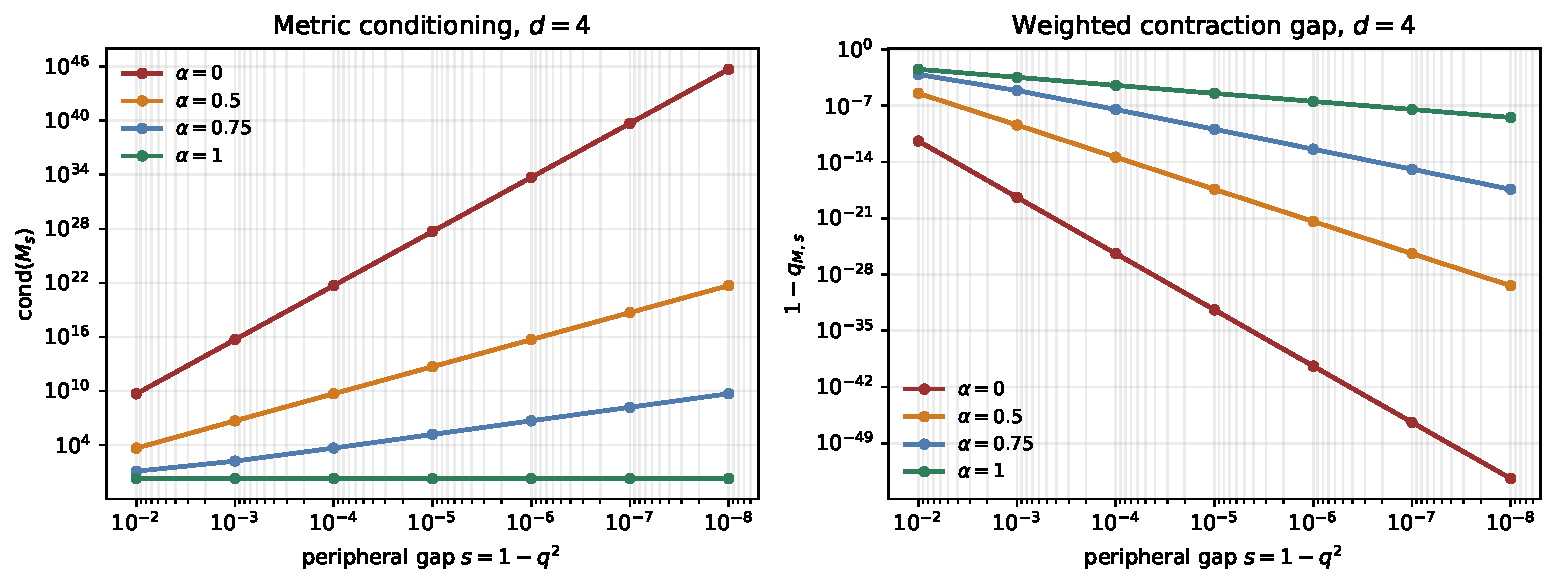
\includegraphics[width=0.98\textwidth]{figures/physical_family_metric_conditioning.pdf}
\caption{Dimension-four coupling laws $c_s=0.2s^\alpha$.  Below the
gap-scale threshold, conditioning grows and the weighted contraction gap
loses exactly one additional power for every conditioning power.}
\label{fig:conditioning}
\end{figure}

At $s=10^{-4}$, the 256-bit Arb audit certifies the exact two-step
Lyapunov identities and positivity.  For fixed $c=0.2$, it certifies
$\cond(M_s)>10^7$ and $1-q_{M,s}<10^{-10}$.  For matched
$c=0.2s$, it certifies $\cond(M_s)<2$ and
$0.4<(1-q_{M,s})/s<0.5$.  These are interval-certified family points, not a
production interval theorem.

\section{Route consequence}
\label{sec:route}

The result closes one ambiguity in RH-64.  Recomputing a canonical metric on
the full near-peripheral space is not a uniform cure: above the coupling-gap
threshold it introduces polynomial or super-polynomial costs, and at the
threshold it still sees the original slow time scale.  This is a negative
result for the order
\[
 \text{full physical space}\longrightarrow\text{one global metric}
 \longrightarrow\text{tail}.
\]

It does not obstruct three narrower constructions:
\begin{enumerate}[leftmargin=2.2em]
 \item use Krylov projection to remove the reached slow directions before
       building the terminal metric;
 \item use block metrics whose coupling is measured relative to each local
       spectral gap;
 \item use observation-weighted Gramians that ignore invisible global
       directions.
\end{enumerate}
The next gate is therefore a block, cross-column Krylov Gram certificate.
It must retain the coherent phase fusion of RH-58--RH-60 while applying
RH-64 only to the final localized residual blocks.

\section{No arithmetic or Hilbert--Polya conclusion}

This paper constructs no self-adjoint operator, no $T\log T$ counting law,
no prime-power trace formula, and no completed-zeta identity.  It makes no
Hilbert--Polya or Riemann-hypothesis claim.  Stage A1 and unconditional Stage
A4 remain open.

\section{Reproducibility}

The directory contains the high-precision solver, tests, family pilot, Arb
audit, figures, hashes, and publication artifacts.  The principal commands
are:
\begin{verbatim}
pytest -q -p no:cacheprovider
python experiments/run_family_conditioning_pilot.py
python experiments/run_arb_two_step_audit.py
MPLBACKEND=Agg python experiments/make_figures.py
latexmk -pdf -interaction=nonstopmode -halt-on-error main.tex
\end{verbatim}

The matrix identities and bounds are analytic.  The fitted exponents are
high-precision finite-family evidence.  Uniform folded-Gaussian metric
conditioning, block cross-column fusion, Stage A1, unconditional Stage A4,
a self-adjoint Hilbert--Polya operator, an arithmetic trace formula, and a
zeta-zero identity remain open.

\bibliographystyle{plainnat}
\bibliography{references}
\end{document}
